%-----------------------------------------------------------------------------------------------------------
% Everything before \begin{document} and
% \end{document} is called Preamble. The Preamble
% sets up your document. The preamble typically specifies
%   the document class
%   languages
%   imports packages by using \usepackage{package_name} command
%-----------------------------------------------------------------------------------------------------------

%-----------------------------------------------------------------------------------------------------------
% Note: A latex command consist of a backslash, command name, argument (with {}) #
% and optional arguments (with []), e.g.
% \command_name[optonal_argument1, optional_argument2 ..]{arugment}
%-----------------------------------------------------------------------------------------------------------

%-----------------------------------------------------------------------------------------------------------
% \documentclass have to be the first command of each latex file and 
% defines layout and class of the document.
%   [options]: contains options to define the layout of the document (fontsize, paper, columns ...) 
%   {class}: defines the class of the document. Possible classes are:
%               - article: for scientifc journals
%               - book: for books
%               - reports: for longer reports with several chapters, thesis, small books
%               - letter: for letters
%               - slides: for slides
%               - beamer: for latex presentations
%   Sources: 
%       https://texblog.org/2013/02/13/latex-documentclass-options-illustrated/ (for options)
%       https://en.wikibooks.org/wiki/LaTeX/Document_Structure#Document_classes (for classes)
%-----------------------------------------------------------------------------------------------------------
\documentclass[a4paper,11pt,onecolumn]{report}

%-----------------------------------------------------------------------------------------------------------
% The \usepackage{package_name} commands imports external packages (here: graphicx)
% to provide latex with external features.
%-----------------------------------------------------------------------------------------------------------
% graphicx package contains commands and features to import external graphic file, i.e.
%   - \includegraphics{picture_name} command to import graphics.
%   - \graphicspath{{path/to/your/images/}} command to tell latex where the graphics are located
\usepackage{graphicx}
\graphicspath{{images}}



%-----------------------------------------------------------------------------------------------------------
% For adding a title, author and date, latex need to include first the following three commands
% in preamble. In a second you have to include the \maketitle command between \begin{docuemtn} and
% \end{document}
%-----------------------------------------------------------------------------------------------------------
% adds a title
\title{Soccer is great \& Politics sucks!}   
% adds a author with footnote to thank, e.g. your institution or coworker
\author{Sefa Kutlu!\thanks{Thanks to Albert Einstein whose shared his great knowledge with us. }}
% adds a date (\today for todays date or a apsicifc date, e.g. \date{August 2022})
\date{\today}                           

%-----------------------------------------------------------------------------------------------------------
% The content of a document have to be added between the \begin{document} and \end{document}
%-----------------------------------------------------------------------------------------------------------
\begin{document}
    % \maketitle commands adds the information defined above with title, author date commands to the document
    % have to be the first command within \begin{document} and \end{document}
    \maketitle
    Hello Latex!. This is an example sentence written by me.
    % \\ new line without new paragraph command
    \\
    % bold, italic, underline commands
    % \textbf{word}: The word in braces will displayed bold
    The last word should be \textbf{bold}.      
    \\
    % \textit{word}: The word in braces will displayed italic
    The last word should be \textit{italic}.
    \\
    % \underline{word}: The word will be underlined
    The last word should be \underline{underlined}.
    \\
    % combine of the three commands from above
    The last three words should be \textbf{\textit{\underline{bold italic underlined}}}.
    \\
    % \emph{argument} effect on its argument will depends on the context, i.e.
    % the emphasized text italicized, but behaviour is reversed inside italic text
    This sentence contains an \emph{emphasized word}, but the rest of the text remains normal.
    \\
    \textit{This italic sentence contains a not italic \emph{word}}
    \\
    % \emph{argument} inside a bold sentence the emphasized word is displayed italic
    \textbf{This bold sentence contains an emphasized \emph{word}}.
    \\

    % It isn't compelling to wrap the \includegraphics{your_file} between
    % \begin{figure} and \end{figure}, but advisable to add a label and caption 
    % to the graphic.
    \begin{figure}
        % \centering command centers the graphic.
        \centering
        % \includegraphics loads the image besiktas_team
        % \textwidth command returns the width of a text on a page
        % [width=\textwidth] option adjusts the width of graphic to the textwidth
        % instead of using \textwidth you can specifiy a specific width with cm, inch ..., e.g.
        % width=2.3cm
        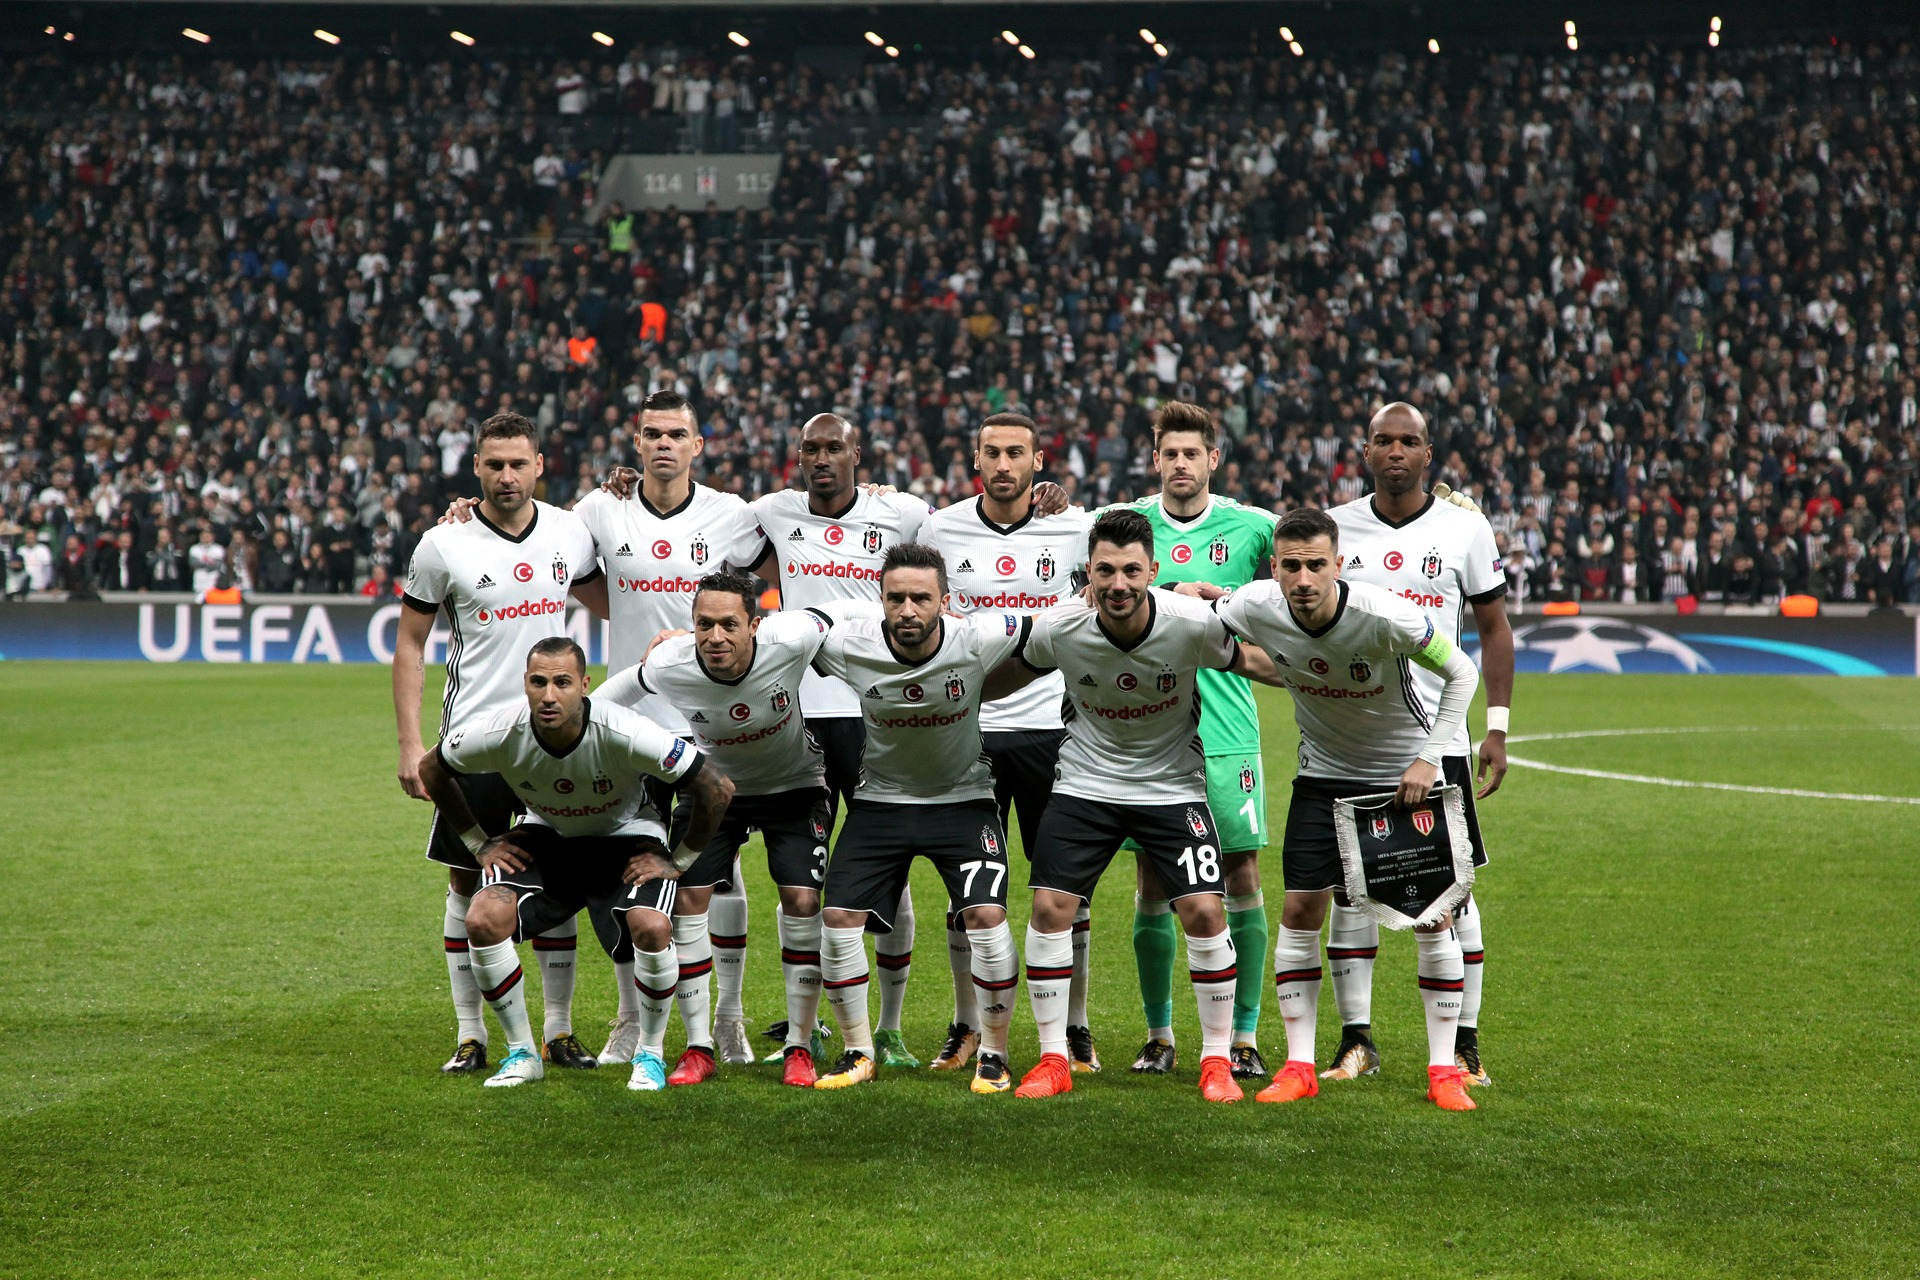
\includegraphics[width=0.75\textwidth]{besiktas_team} % sets width to 75% of textwidth
        % \caption{arg} command gives the figure a caption
        \caption{Besiktas JK 2017/2018}
        % \label{fig:<name>} command labels the figure and generates a number to reference the image within the document
        % with \ref{fig:<name>}
        % \label command have to be the last in a figure, otherwise the reference won't displayed.
        \label{fig:besiktas_team}     
    \end{figure}

    % This \includegraphics command can contain following options, comment or comment out the options you want
    % to try out.
    \begin{figure}
        \centering
        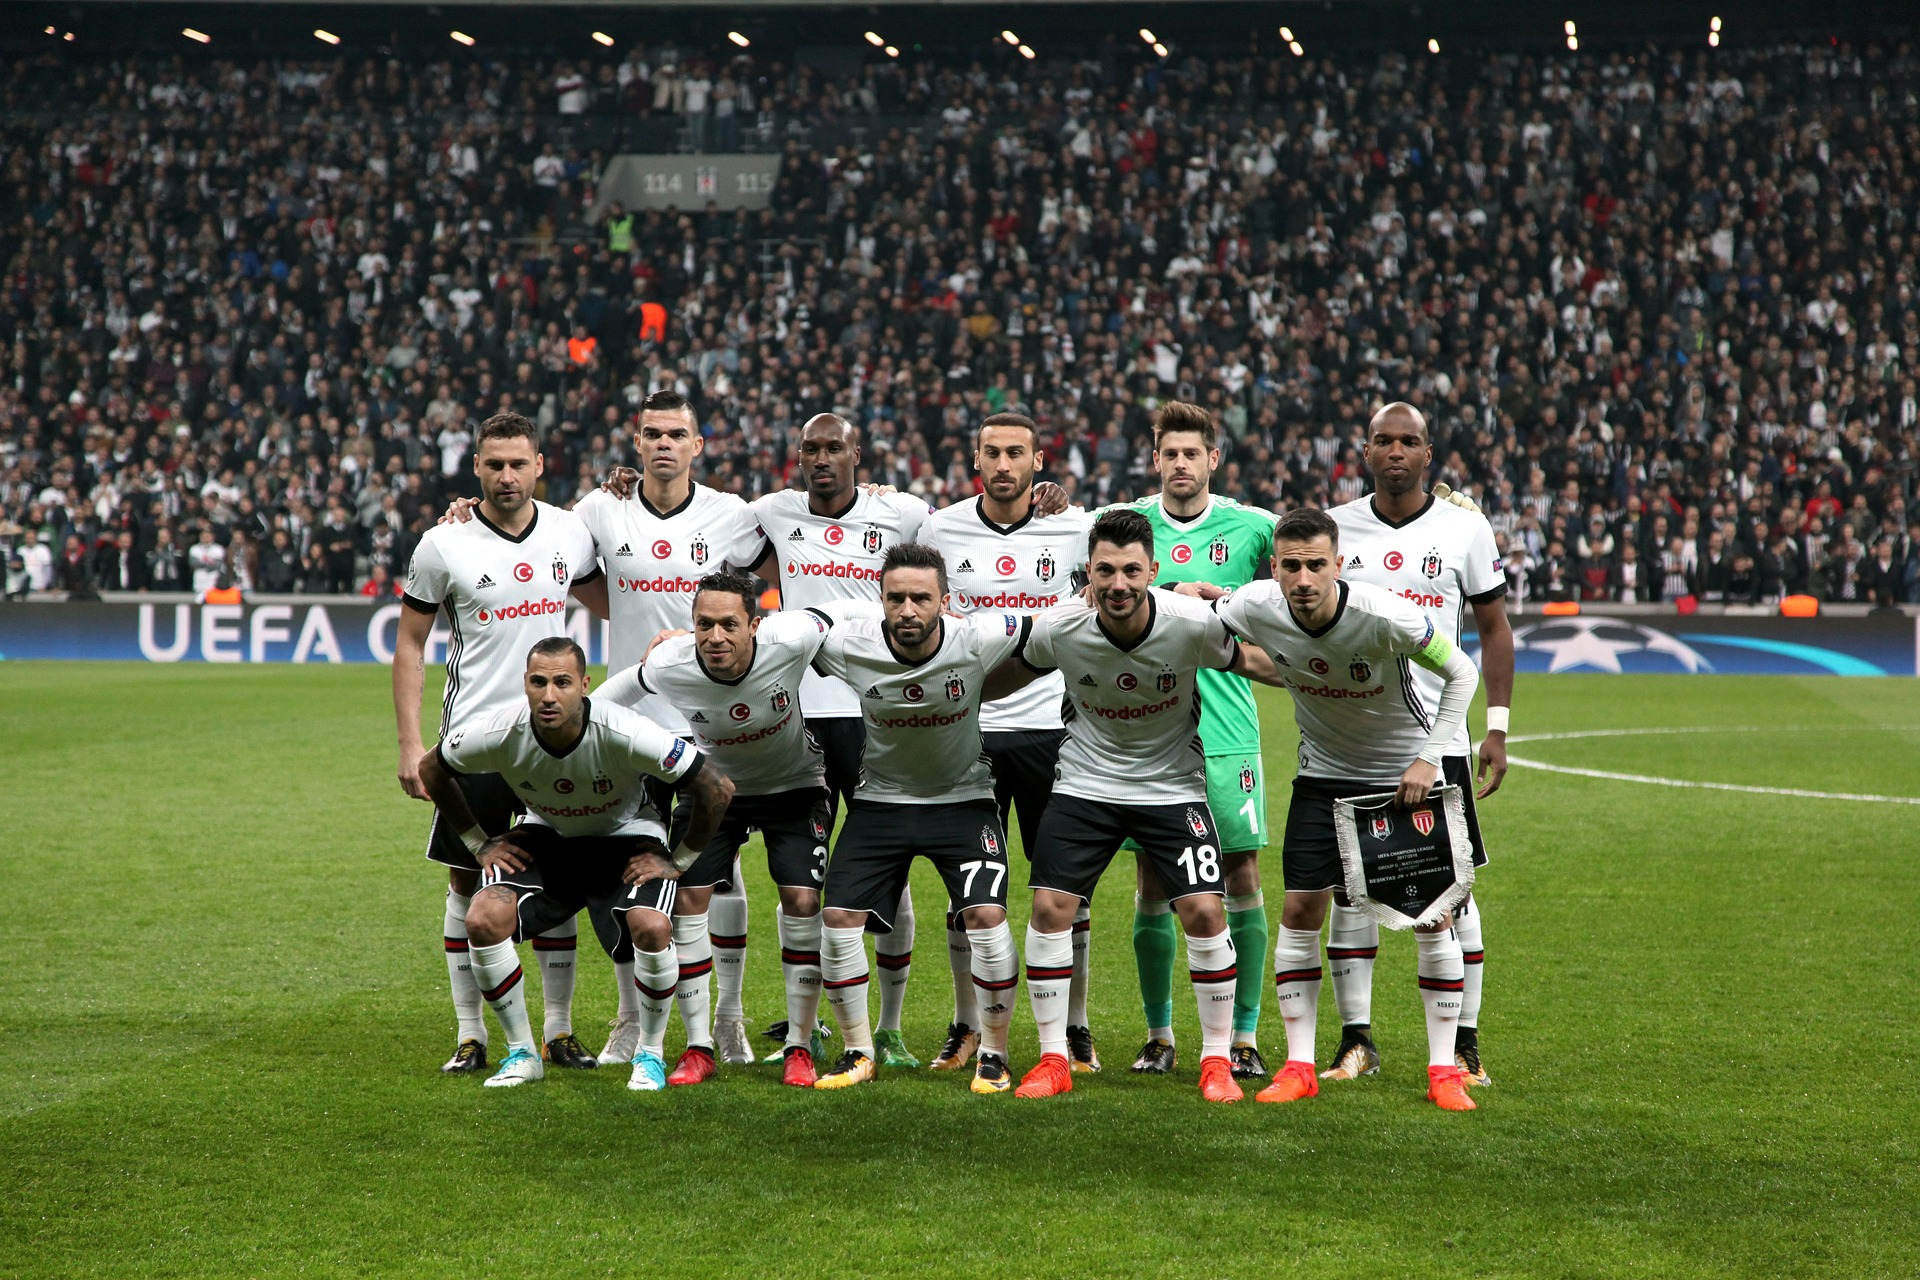
\includegraphics
        [%scale=0.10,% scale scales graphic based on specified scale factor
         %width=5.5cm,% width scales graphic based on specified width 
         height=3.5cm,% height scales graphic based on specified height
         %draft % is draft set, latex displays a placeholder (path of file) instead of loading the image. Accelerates the translation process of document.
         angle=-90,% angle rotate the graphic based on specified value, positiv values = counterclockwise, negative values = clockwise,
         % -90 rotates the graphics 90 degree clockwise
        ]{besiktas_team}
        \caption{height 3.5cm and rotate -90 degree (clockwise)}
        \label{fig:besiktas_team_with_several_options}
    \end{figure}

    % \ref{figure} command is substituted by the number corresponding to the referenced figure 
    % \pageref{figure} command is substituted by the page number on which the figure is displayed.  
    The Figure \ref{fig:besiktas_team} is on page \pageref{fig:besiktas_team}.

    \clearpage

    %----------------------
    %   Lists
    %----------------------
    % An unordered list is created with the enviroment \begin{itemize} ... \end{itemize}
    % and items are defined inside them with: \item example item 
    % for example:
    \begin{itemize}
        \item an item
        \item another item
        \item useless item
    \end{itemize}
    
    % An ordered list is created with the enviroment \begin{enumerate} ... \end{enumerate}
    % and items are defined inside them with: \item example item 
    % for example:
    \begin{enumerate}
        \item first item
        \item second item
        \item third item
    \end{enumerate}

    %----------------------
    %   Math
    %----------------------
    % A Huge advantage of Latex is the ease of writing mathematical expressions.
    % There are two modes to write mathematical expression:
    % 1. inline math mode: used to write formulas that are part of a paragraph
    % 2. display math mode: used to write formulas that are not part of text or paragraphs
    % and are set on separate lines.

    % Inline math mode
    % To typeset inline math mode u can use one of the these delimiter pairs:
    % \(...\)
    % $...$
    % \begin{math}...\end{math}
    The following commands demonstrate how you can typeset inline-mode math.\\
    % \textbackslash command creates a \ within text, it can't be used as \ in a text, since 
    % it is a special character reserved for latex commands.
    % Special characters reserved by latex can be used in text with \ before the character
    % e.g. \{ = { (in text), \] = ] (in text).
    With \textbackslash begin\{math\} \dots \textbackslash end\{math\}.
    \begin{math}
        E=mc^2
    \end{math}
    \\
    With \$\dots\$
    $E=mc^2$
    \\
    With \textbackslash (\dots\textbackslash)
    \(E=mc^2\)

    % Display math mode
    % To typeset display-mode math u can one of these delimiter pairs:
    % \[...\]
    % \begin{displaymath} ... \end{displaymath}
    % \begin{equation} ... \end{equation}
    The following commands demonstrate how you can typeset display-mode math
    Here comes some text. Let's see if the formulas 
    \[E=mc^2\]
    \begin{displaymath}
        E=mc^2
    \end{displaymath}
    \begin{equation}
        E=mc^2
    \end{equation}
    will appear in this paragraph
    or in a new line.

    % More Complex Math
    % _ for subscripts
    % ^ for Superscripts
    Subscripts (dt. index) in math mode are written as $a_b$ (\$a\_b\$). \\
    Superscripts (dt. exponent) in math mode are written as $a^b$ (\$a\^{}b\$). \\

    % Example for complex math formulas
    % \dots command displays ...
    % Hint: Group subscripts & Superscripts with multiple variables or numbers
    % inside {...}
    \[T^{i_1i_2 \dots i_p}_{j_1,j_2 \dots j_q} = 
    T(x^{i_1},\dots,x^{i_p},e_{j_1},\dots,e_{j_q})\]

    % Integrals are written with the \int command.
    % Append \int ^<char>_
    Integrals are written by using \textbackslash int command. You can
    append, e.g. \^{}5\_1 to define 5 as upper and 1 as 
    lower boundary. Also, possible to append it in the revert order like 
    \_{}1\^{}5. Both will produce the same output. 
    \[\int^5_1\]
    \[\int_1^5\]


    Fractions are written by using \textbackslash frac\{Numerator\}\{Denominator\}, e.g.
    \begin{displaymath}
        \frac{Numerator}{Denominator}
    \end{displaymath}

    The following formula describes using the \textbackslash int and
    \textbackslash frac \{Numerator\}\{Denominator\}
    \begin{equation}
        \int^1_0 \frac{dx}{e^x} = \frac{e-1}{e}    
    \end{equation}

    % Example for lower- and uppercase greek letters
    % lowercase leters
    \clearpage
    Example for lowercase Greek letters.
    \begin{itemize}
        \item $\omega$
        \item $\delta$
        \item $\gamma$
        \item ...
    \end{itemize}

    Example for uppercase Greek letters
    \begin{itemize}
        \item $\Omega$
        \item $\Delta$
        \item $\Gamma$
        \item ...
    \end{itemize}
    Greek letters have their own commands (e.g.\textbackslash omega for $\omega$). To produce lowercase Greek
    letters you have to write the corresponding command of the letter in 
    lowercase. For the uppercase Greek letters you have write the first
    letter of the command in uppercase.\\

    % Example for sin, cos and log
    Example for sin, cos and log, Attention: NEVER FORGET TO PUT MATH FORMULAS
    BETWEEN MATH MODE COMMANDS!!!.
    \begin{itemize}
        \item $\sin(\beta)$, latex command:  \$\textbackslash sin(\textbackslash beta)\$ 
        \item $\cos(\alpha)$, latex command:  \$\textbackslash cos(\textbackslash alpha)\$ 
        \item $\log(x)$, latex command:  \$\textbackslash log(x)\$ 
    \end{itemize}

    % Math square root 
    Example for square root. The command: \textbackslash sqrt\{expression\}
    \[\sqrt{x^2+1}\]

\end{document}


%-----------------------------------------------------------------------------------------------------------
% Sources:
%           https://www.overleaf.com/learn/latex/Learn_LaTeX_in_30_minutes#The_preamble_of_a_document
%           
%           
%           
%           
%           
%           
%           
%           
%           https://pixabay.com/photos/besiktas-sho-champions-league-2910497/ (picture: besiktas_team)
%           https://pixabay.com/photos/soccer-europe-uefa-champions-league-2698966/ (picture besiktas_flag)
% 
%
%
% 
%
%
% 
%
%
% 
%
%
% 
%
%
% 
%
%
% 
%-----------------------------------------------------------------------------------------------------------
